\documentclass[handout]{beamer}
\usepackage{beamerthemesplit}
\usepackage{pgfpages}

\usepackage{tikz}
\usetikzlibrary{arrows,%
                shapes,positioning}

\tikzstyle{vertex}=[circle,fill=black!25,minimum size=20pt,inner sep=0pt]
\tikzstyle{selected vertex} = [vertex, fill=red!24]
\tikzstyle{edge} = [draw,thick,-]
\tikzstyle{weight} = [font=\small]
\tikzstyle{selected edge} = [draw,line width=5pt,-,red!50]
\tikzstyle{ignored edge} = [draw,line width=5pt,-,black!20]

\usetheme{Madrid}
\title[Multi-Cast Key Management Protocols]{Multi-Cast Key Management Protocols \\ Design, Specification, and Analysis}

\usepackage{mathptmx}
\usepackage[scaled=.90]{helvet}
\usepackage{courier}
\usepackage[T1]{fontenc}

%%\pgfpagesuselayout{4 on 1}[letterpaper,border shrink=5mm]

\institute[RIT]{}
\date{February 3, 2012}
%\subtitle{}
\author{Christopher A. Wood}
%\institute[]{}
%\date{}
\begin{document}

\begin{frame}
  \titlepage
  \begin{center}
	  %\textbf{caw4567@rit.edu}
	\end{center}
\end{frame}

\begin{frame}
	\frametitle{Agenda}
 	\begin{enumerate}
	\item Project goal
	\item Review group key management problem
	\item Protocol design limiting constraints 
	\item Viral protocol design and performance
	\item ARK protocol design performance
	\end{enumerate}
\end{frame}

\begin{frame}
	\frametitle{Project Goal}
	Develop a practical method to support tactical group key establishment
\end{frame}

\begin{frame}
	\frametitle{Group Key Management Problem}
	\begin{itemize}
	\item Existing PKI based EKE and Authentication methods are inherently PtP protocols
	\item Previously proposed solutions to group and multi-case applications are limited
		\begin{itemize}
		\item Most require the presence of a trusted server or network manager
		\item PtP transactions can require up to 9 symmetric exchanges
		\item Non-PtP based methods involve a great deal of pre-placed information
		\end{itemize}
	\item Need to be secure against common attacks (e.g. Man in the Middle)
	\end{itemize}
\end{frame}

\begin{frame}
	\frametitle{Group Key Management Problem}
	\begin{itemize}
	\item Lack of pre-placed information calls for solutions with strong PKI-based Electronic Key Exchange (EKE) mechanisms
	\item EKE techniques suffer from the need for large key sizes
	\item Standardized EKE mechanisms are traditionally sequential for SA establishment among peers
	\item A complete EKE capability is required to enable widespread adoption by the military customer
	\end{itemize}
\end{frame}

\begin{frame}
	\frametitle{Multi-Cast Key Management}
 	\begin{center}
  	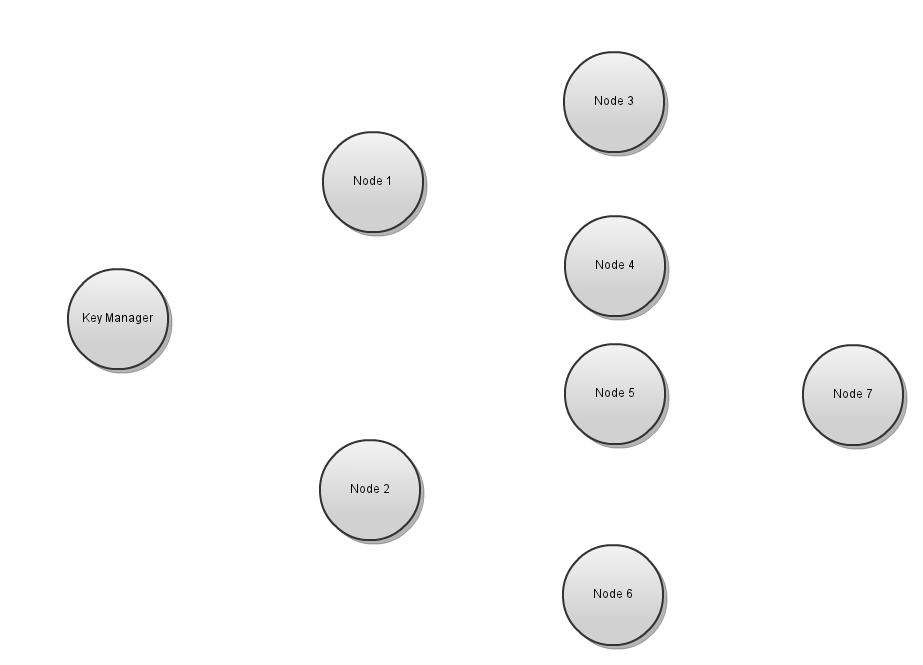
\includegraphics[width=85mm]{NodeGroup.jpg}
 	\end{center}
\end{frame}

\begin{frame}
	\frametitle{Multi-Cast Key Management}
	\begin{center}
 	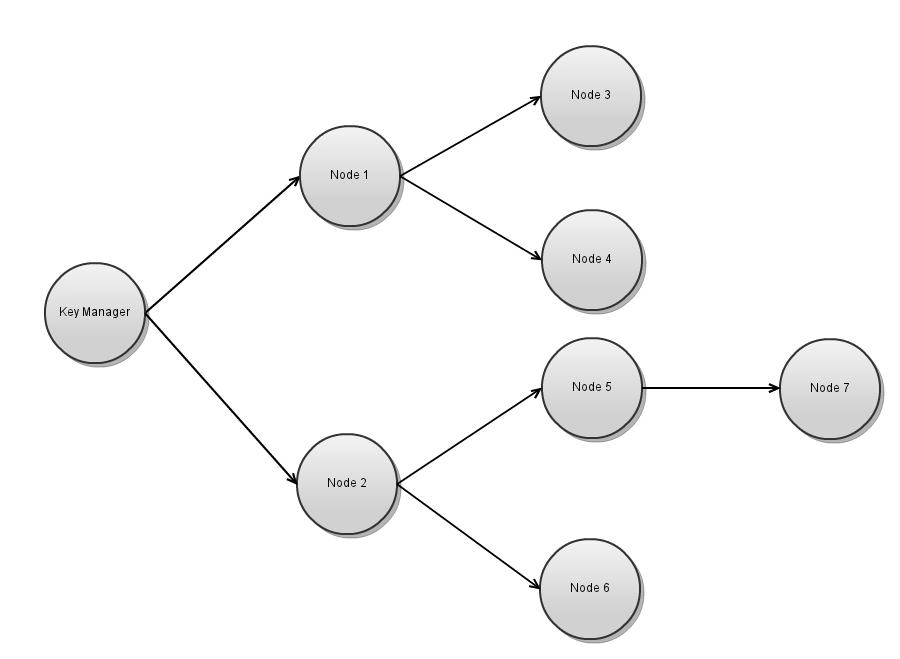
\includegraphics[width=85mm]{SpanTree.jpg}
	\end{center}
\end{frame}

\begin{frame}
	\frametitle{Multi-Cast Key Management}
 	\begin{center}
 	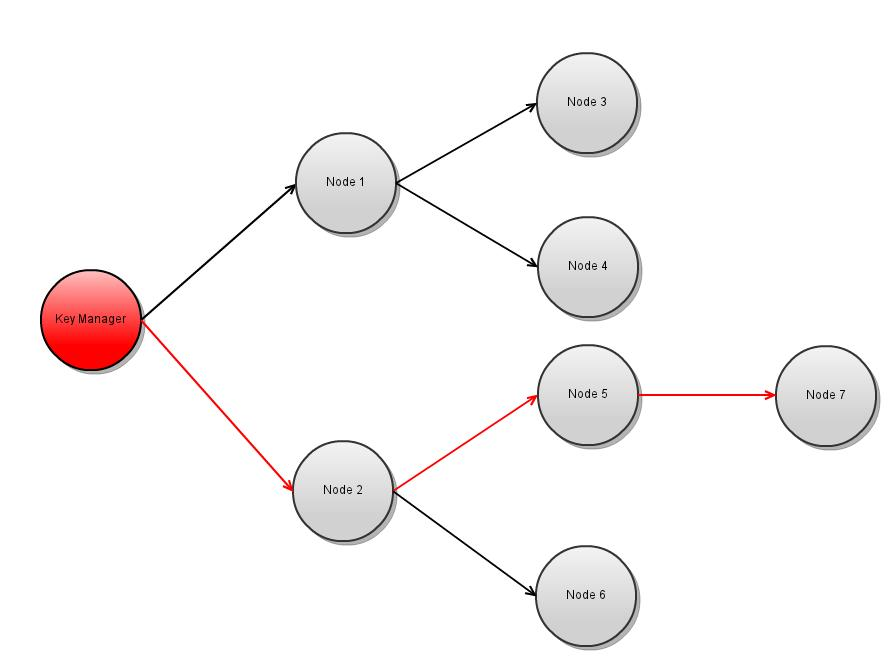
\includegraphics[width=85mm]{SpanTreeHighlight.jpg}
	\end{center}
\end{frame}

\begin{frame}
	\frametitle{Design Constraints}
	\begin{enumerate}
	\item Wireless channel is bandwidth constrained
	\item Radio units are somewhat computationally constrainted
	\item Limitations on shared secret and pre-placed information
	\item Group membership can consist of the entire battlefield
	\item Adding group members is easy, removing them requires full network rekey
	\end{enumerate}
\end{frame}

\begin{frame}
	\frametitle{Proposed Solutions}
	Two different protocols for targeting different deployment settings (wideband/multiband and narrowband channels)
	\begin{enumerate}
	\item Viral EKE Protocol
	\item ARK EKE Protocol
	\end{enumerate}
\end{frame}

\begin{frame}
	\frametitle{Viral EKE Protocol - Design Principles}
	\begin{itemize}
	\item Re-key events are triggered from a single key manager, but the work is partially offloaded to the rest of the group
		\begin{itemize}
		\item Key manager role is propogated throughout the members of the group to form pariwise security associations (SAs) that are then used to distribute the session key
		\item Pairwise SA establishment can be done in parallel with members throughout the group
		\end{itemize}
 	\item Parallel implementation of the standardized Internel Key Exchange (IKE) protocol for ad-hoc group re-keys
		\begin{itemize}
		\item Allows overhead of each exchange to be distributed among all members of the group
		\end{itemize}
	\item Closely tied to the underlying data-link layer spanning tree orientation of groups to perform key distribution
	\item Support for an AUL to determine valid nodes is being integrated into the scheme
	\end{itemize}
\end{frame}

\begin{frame}
	\frametitle{Viral EKE Protocol - Targets}
	\begin{itemize}
	\item Targeted towards wideband and multiband networks
		\begin{itemize}
		\item AN/PRC-117G, 30 Mhz - 2 Ghz RF channel bandwidth
		\item SATCOM, Wideband (WB)
		\item Data rates
			\begin{itemize}
			\item On-air rates up to 10 Mbps
			\end{itemize}
		\end{itemize}
	\end{itemize}
\end{frame}

\begin{frame}
	\frametitle{Viral EKE Protocol - Exchange Paths}
 	\begin{center}
 	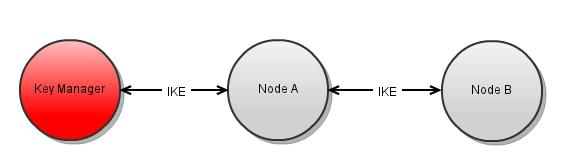
\includegraphics[width=85mm]{Viral_group.jpg}
	\end{center}
\end{frame}

\begin{frame}
	\frametitle{Viral EKE Protocol - Exchange Paths}
 	\begin{center}
 	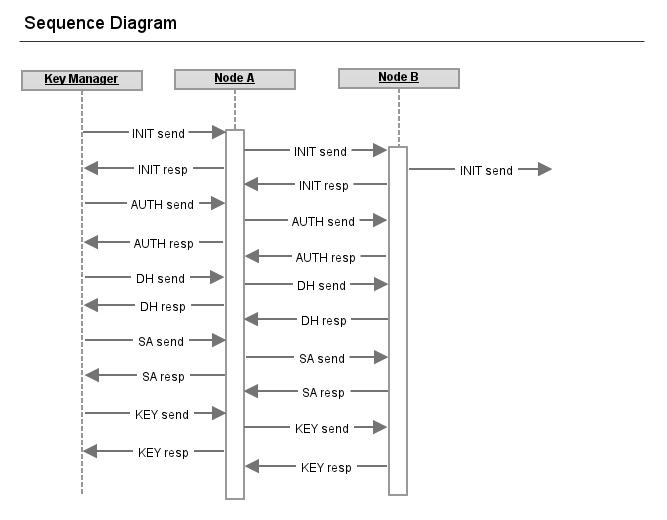
\includegraphics[width=85mm]{Viral_sequence.jpg}
	\end{center}
\end{frame}

%\begin{frame}
%	\frametitle{Viral EKE Protocol - Simulated Performance Results}
%	\begin{itemize}
%	\item TODO: plop some charts here
%	\end{itemize}
%\end{frame}

%\begin{frame}
%	\frametitle{Viral EKE Protocol - Simulated Performance Results}
%	\begin{itemize}
%	\item TODO: plop some charts here
%	\end{itemize}
%\end{frame}

\begin{frame}
	\frametitle{Viral EKE Protocol - Performance Review}
 	\begin{itemize}
	\item The group re-key time grows logarithmically with the number of allowed children in the transaction spanning tree
	\item Balanced spanning tree orientations with limited children nodes result in highest performance benchmarks
	\end{itemize}
\end{frame}

\begin{frame}
	\frametitle{ARK EKE Protocol - Design Principles}
	\begin{itemize}
 	\item Automatic group key management with utilization of a one-way cryptosystem for key exchanges over the air
		\begin{itemize}
		\item An asymmetric cipher is used with both the encryption and decryption key kept secret
		\item This creates three kinds of users in the group
			\begin{itemize}
			\item Sender -  A member who can only encrypt messages
			\item Receiver - A member who can only decrypt messages
			\item Intruder - A member who possesses neither the encryption or decryption key and cannot encrypt or decrypt any messages.
			\end{itemize}
		\end{itemize}
	\item Encryption and decryption keys are stored as pre-placed information before the start of a mission
	\item Further pre-placed information (e.g. user authentication lists) can be added for additional security
	\end{itemize}
\end{frame}

\begin{frame}
	\frametitle{ARK EKE Protocol - Targets}
	\begin{itemize}
	\item Targeted towards a tactical HF radio
		\begin{itemize}
		\item 3 and 30 MHz, 3 KHz channels
		\item Data rates
			\begin{itemize}
			\item MIL-STD-188-110B (9600 bps and 12,800 bps uncoded)
			\end{itemize}
		\end{itemize}
	\end{itemize}
\end{frame}

\begin{frame}
	\frametitle{ARK EKE Protocol - Exchange Paths}
 	\begin{center}
 	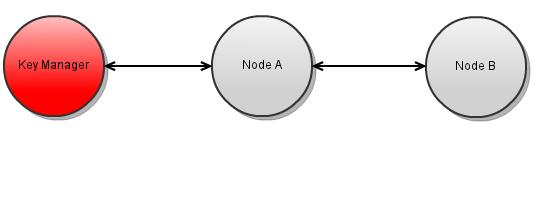
\includegraphics[width=85mm]{ARK_group.jpg}
	\end{center}
\end{frame}

\begin{frame}
	\frametitle{ARK EKE Protocol - Exchange Paths}
 	\begin{center}
 	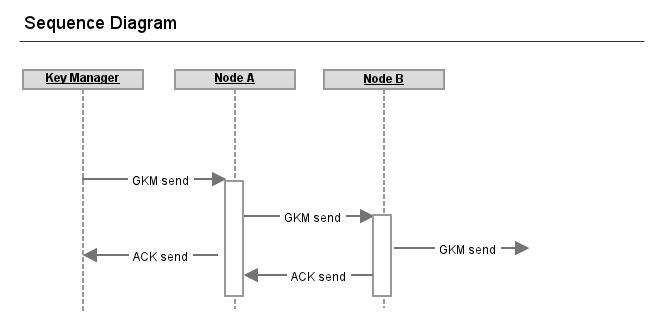
\includegraphics[width=85mm]{ARK_sequence.jpg}
	\end{center}
\end{frame}

%\begin{frame}
%	\frametitle{ARK EKE Protocol - Simulated Performance Results}
% 	\begin{itemize}
%	\item TODO: plop some charts here
%	\end{itemize}
%\end{frame}

%\begin{frame}
%	\frametitle{ARK EKE Protocol - Simulated Performance Results}
% 	\begin{itemize}
%	\item TODO: plop some charts here
%	\end{itemize}
%\end{frame}

\begin{frame}
	\frametitle{ARK EKE Protocol - Performance Summary}
 	\begin{itemize}
	\item The group re-key time grows logarithmically with the number of allowed children in the transaction spanning tree
		\begin{itemize}
		\item Since the group key is distributed in a single packet the prospect of parallel transactions to distribute communication overhead is not as significant as in the Viral technique
		\end{itemize}
	\item Scalable to other target waveforms
		\begin{itemize}
		\item The single group re-key message is all-inclusive and is suitable for any channel bandwidths at the cost of pre-placed information
		\end{itemize}
	\end{itemize}
\end{frame}

\begin{frame}
	\frametitle{Simulation Notes}
 	\begin{itemize}
	\item Manually introduced timing delays on packet transactions
		\begin{itemize}
		\item Avoidance of signal interference
		\item Emulation of TDMA ring access
		\end{itemize}
	\item Computational overhead is estimated 
		\begin{itemize}
		\item Will likely change based on the properties of each physical unit used with each key management technique
		\end{itemize}
	\end{itemize}
\end{frame}

\begin{frame}
	\frametitle{Future Work}
	\begin{itemize}
	\item Formal mathematical analysis of each protocol
		\begin{itemize}
		\item Will be used for comparison with simulated results
		\end{itemize}
	\item Security analysis of each protocol
		\begin{itemize}
		\item Will be used to ensure the structure and content of key exchange messages is appropriate and not susceptible to compromising attacks
		\end{itemize}
	\end{itemize}
\end{frame}

%\begin{frame}
 %\frametitle{Internal node structure}
 %\begin{center}
  %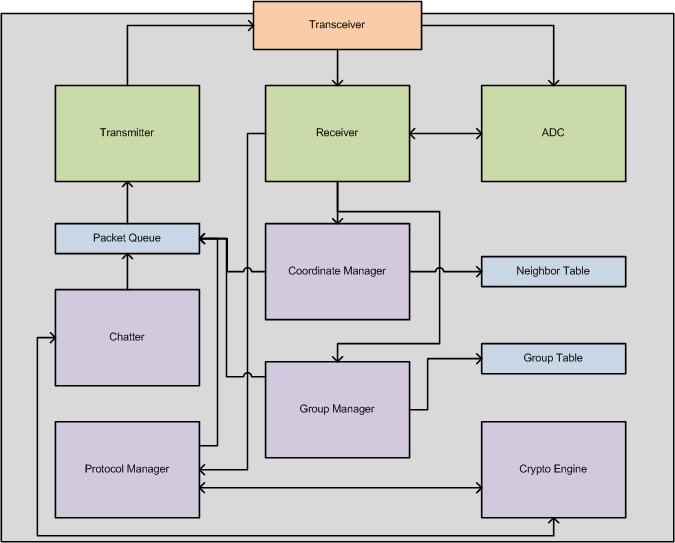
\includegraphics[width=85mm]{dynamic_node.jpg}
 %\end{center}
%\end{frame}

\end{document}